\section{Requirements}
\label{sec:Requirements}

\subsection{Overview} 
The following section is on the requirements of the project and development methodology. 

\subsection{Development Methodology}
The stakeholders for this project is the project owner and sponsor, project advisor, and developer, Claire Mitchell, Elliott Forbes, and Austin Klum respectively. The end users are the students using the virtual reality tool for their learning and the instructors using the quiz management tool for assessment of student's comprehension of classroom material.
\\
The chosen development methodology for a project is an early and influential decision made that alters the course of development. As this was a solo-developer, web, and virtual reality project with a busy project sponsor, the decision was made to make use of an iterative agile methodology. An iterative agile approach focuses on delivering value to the product in fast small increments, rather than all at once. This approach allows software developers to adjust, refine, and review the development process to better provide value and output. This approach also allows for earlier risk identification and the flexibly to easily correct course.\\
\\
Traditional methodology follows the waterfall approach which \qquote{contains five phases of management, where each requires a deliverable from the previous phase to proceed}{waterfall}. The waterfall method is more suitable for projects that follow a linear path and is fixed and rigid. The project did not have this rigidity or clarity of output, hence a more Agile approach was taken. The developer also made use of a KanBan board to help keep organized which a snippet can be seen in Figure \ref{KanBan}. 

\begin{figure}[htb]
	\centering
	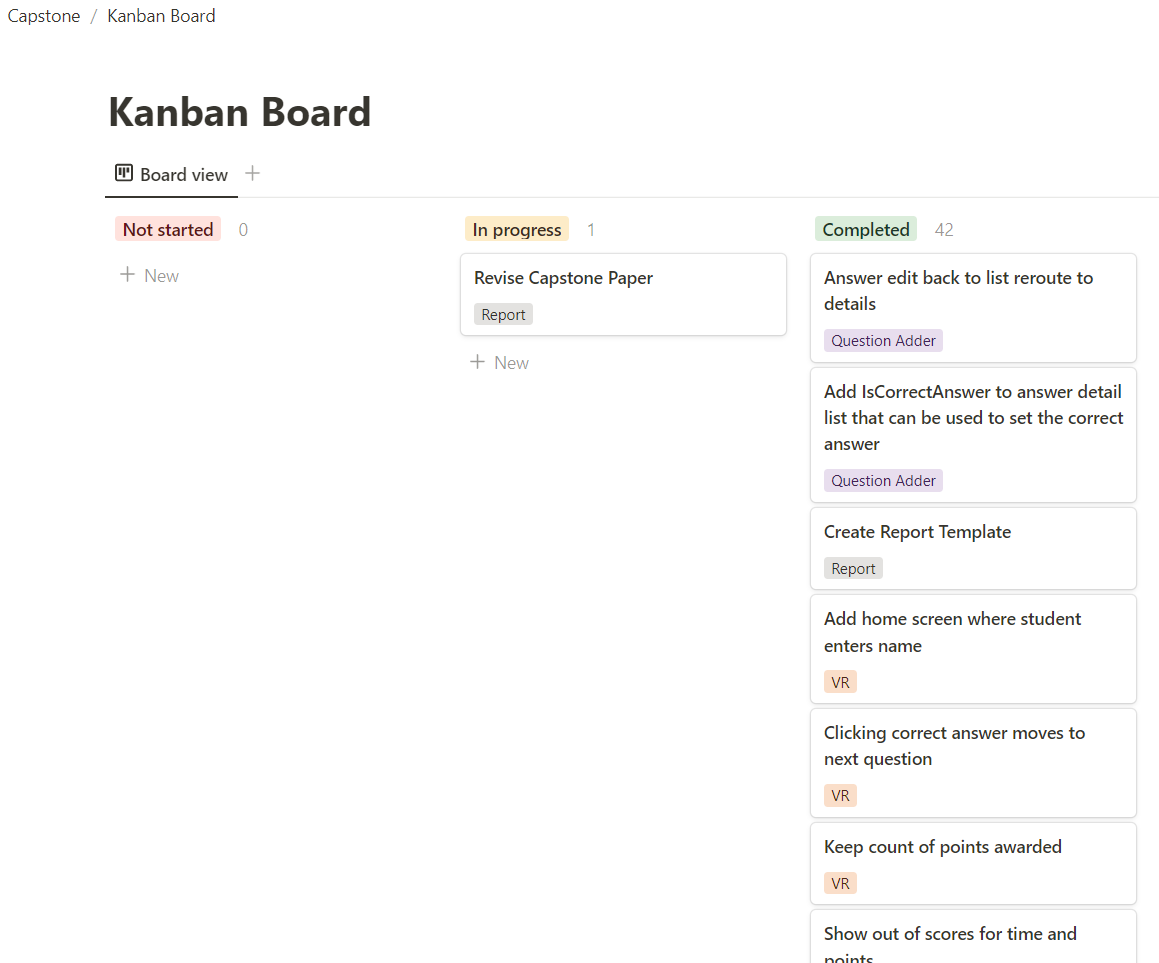
\includegraphics[width=.6\textwidth]{Requirements/assets/KanBan-Board.png}
	\caption[KanBan Board Snippet]{\label{KanBan}KanBan Board Snippet}
\end{figure}

\subsection{Course Creator}
This tool allows the project sponsor and verified users to create orienteering courses for the students to complete. Upon logging in, the verified user views the list of courses available. Each course is comprised of locations which has a corresponding photo to accompany the location. To help with immersion and to best utilize the capabilities of virtual reality, the uploaded photos must be 360 Photos, also known as a photo sphere. This type of photo allows for the virtual reality tool to wrap the image around the user making a sphere, such that the user is able to look around as if they were really at that location. The decision to use 360 Photos was made as the 3D models for the locations aren't available and would limit the locations possible for the courses. This decision enables the verified users to create any course desired as 360 Photos are easy to capture and create. The tool also allows for locations to be added, updated, or deleted. Each location has a list of questions. There is no limit to the number of questions per location. The tool allows for each question to be added, updated, or deleted. Each question has a list of answers which can be of one to six possibilities. The tool allows for each answer to be added, updated, or deleted. \\
\\
Once a course has been completed by a student, a verified user can view the results from the course main dashboard. This dashboard lists the student ID, point score, time score, and total score. As security is important, the database is encrypted and requires an authorized administrator database account to access the data outside of the tool. \\
\\
For a user to be created, they must create an account with an email and password. Once the account is created, the user is immediately able to login, but will be unable to access any of the course creation or course results pages, limited only to the homepage and user settings. Each verified user has the capability to approve other users. In the user settings page, there exists a link to verify users. The verify users page list all users and their status of verified or not verified. From here a verified user can verify or un-verify other users by selecting the corresponding checkbox and saving. 


\subsubsection{Users}
Figure \ref{Course Creator Use Case Diagram} explains the use case diagram. The use cases shows the actions a new user and an verified user can take. A new user is limited to registering, loging in, and update their account. A verified user is able to create, update, and delete courses and subcomponents.

\begin{figure}[htb]
	\centering
	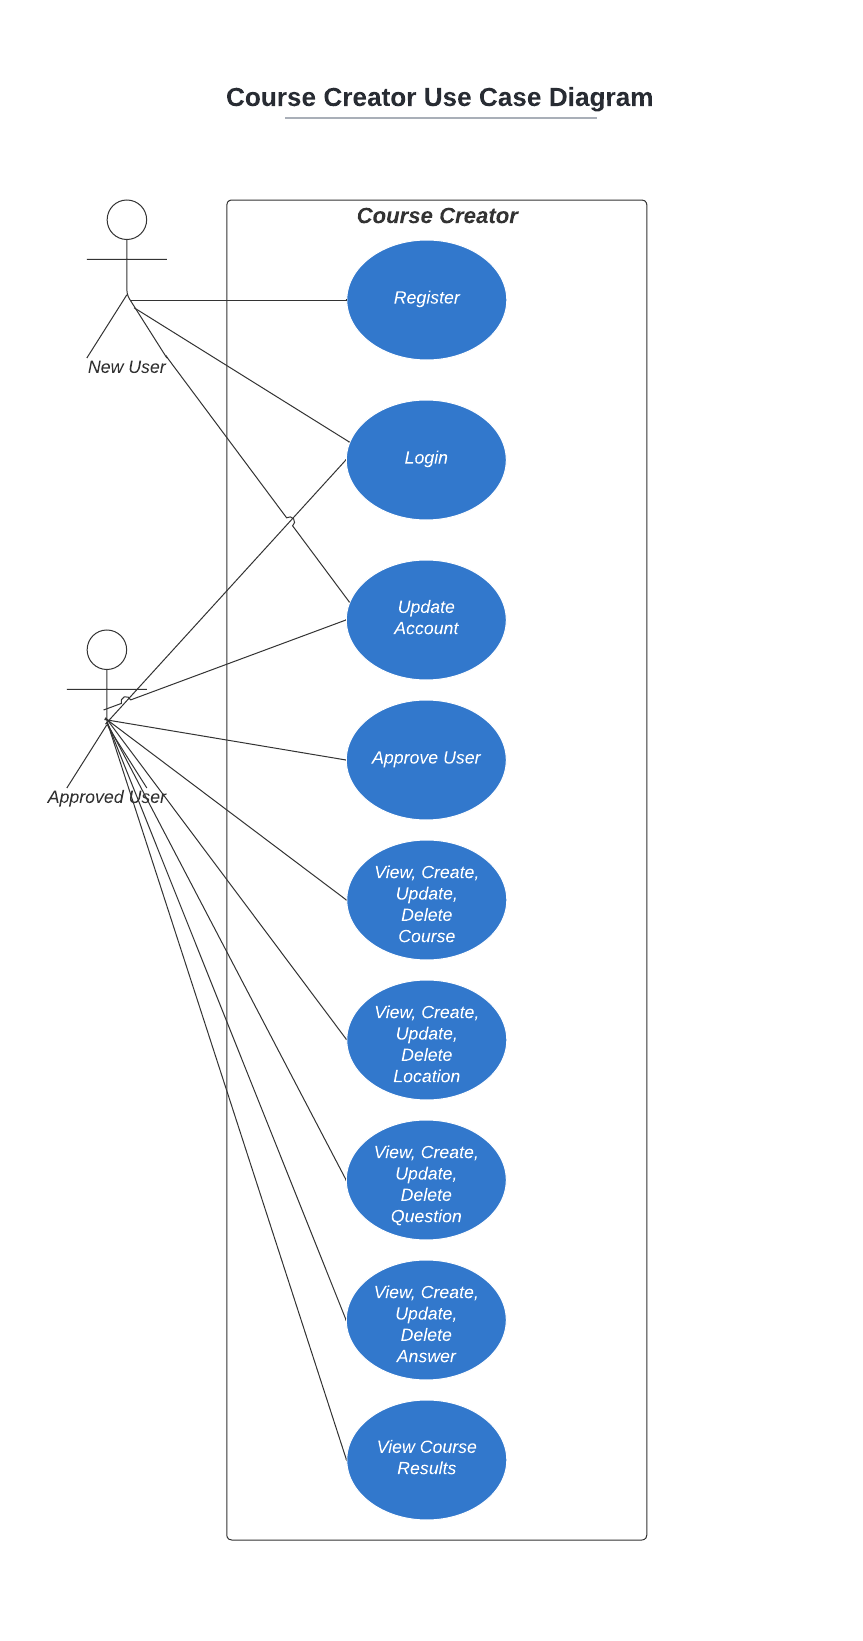
\includegraphics[width=.6\textwidth]{Requirements/assets/course-creator-use-case-diagram.png}
	\caption[Course Creator Use Case Diagram]{\label{Course Creator Use Case Diagram}Course Creator Use Case Diagram}
\end{figure}

\subsubsection{Create Course Flow}
When a user first navigates to the Course Creator they will be required to login to their account or register an account. Figure \ref{Course Creator Login} shows this login screen.

\begin{figure}[htb]
	\centering
	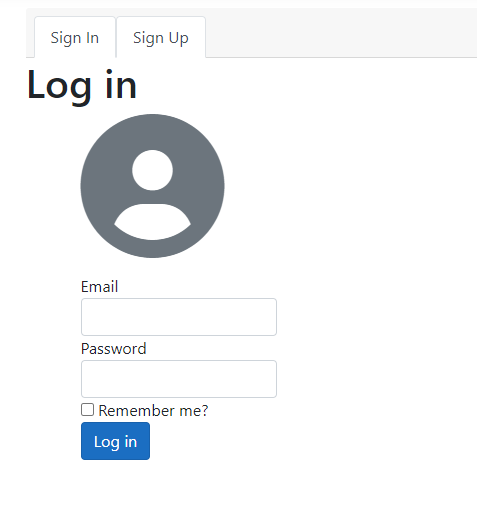
\includegraphics[width=.6\textwidth]{Requirements/assets/cc-login.png}
	\caption[Course Creator - Login]{\label{Course Creator Login}Course Creator - Login}
\end{figure}

Once logged in or registered with a new account, the user is not verified. A non-verified user cannot view, create, update, or delete any of the courses or sub-components. Figure \ref{CC Denied} shows the access denied screen for not verified users. 
\begin{figure}[htb]
	\centering
	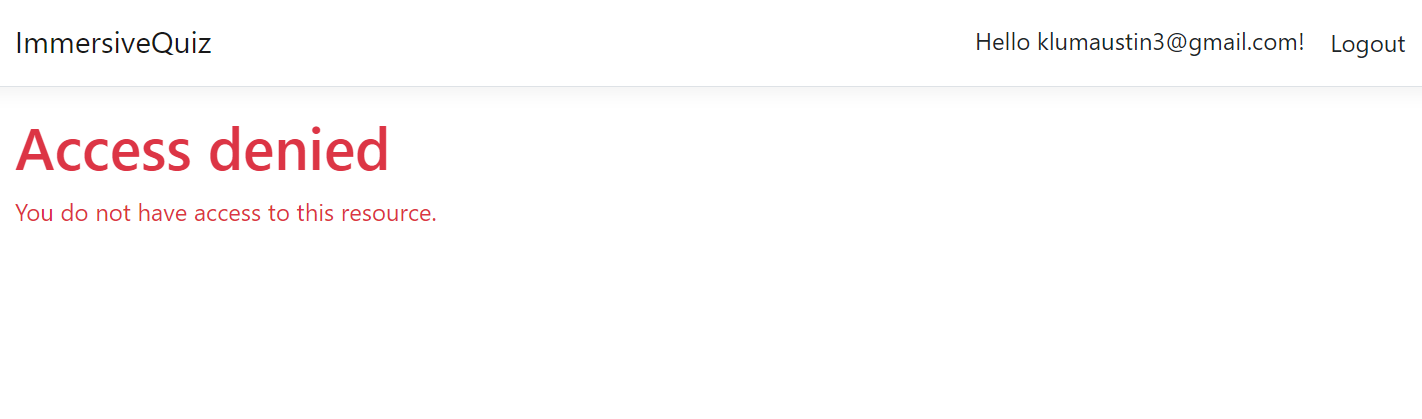
\includegraphics[width=.6\textwidth]{Requirements/assets/cc-access-denied.png}
	\caption[Course Creator - Access Denied]{\label{CC Denied}Course Creator - Access Denied}
\end{figure}
However, a non-verified user can still access they're account details and make changes. For verified users, the account management page also allows for verifying other users. Figure \ref{CC Manage Account} shows a verified users account management page.
\begin{figure}[htb]
	\centering
	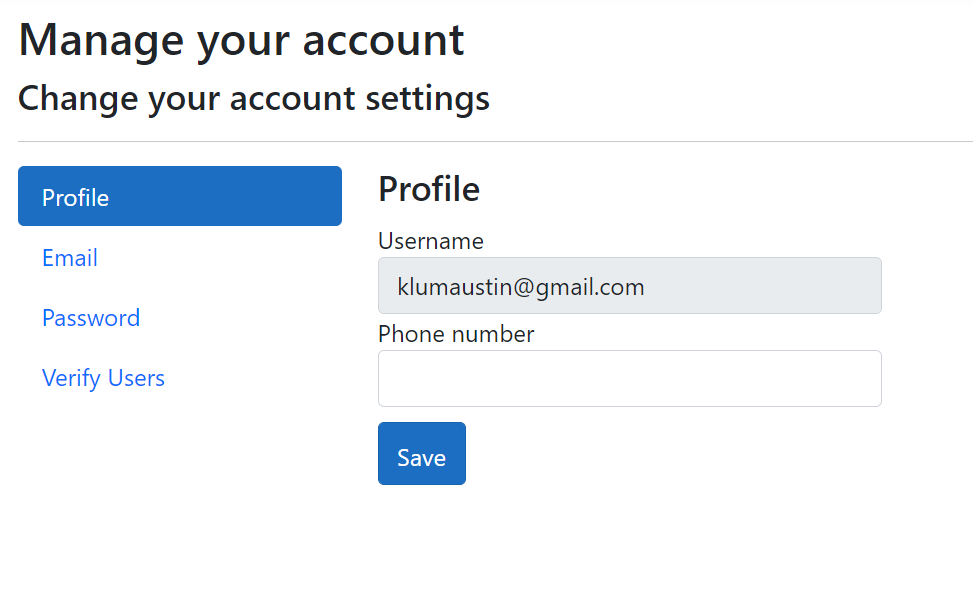
\includegraphics[width=.6\textwidth]{Requirements/assets/cc-manage-account.png}
	\caption[Course Creator - Manage Account]{\label{CC Manage Account}Course Creator - Manage Account}
\end{figure}
When a verified user accesses the verify users page the user is presented with the list of users who are not verified and verified. From here a verified user can verify non-verified users. Figure \ref{CC Verify} shows the verify user page. 
\begin{figure}[htb]
	\centering
	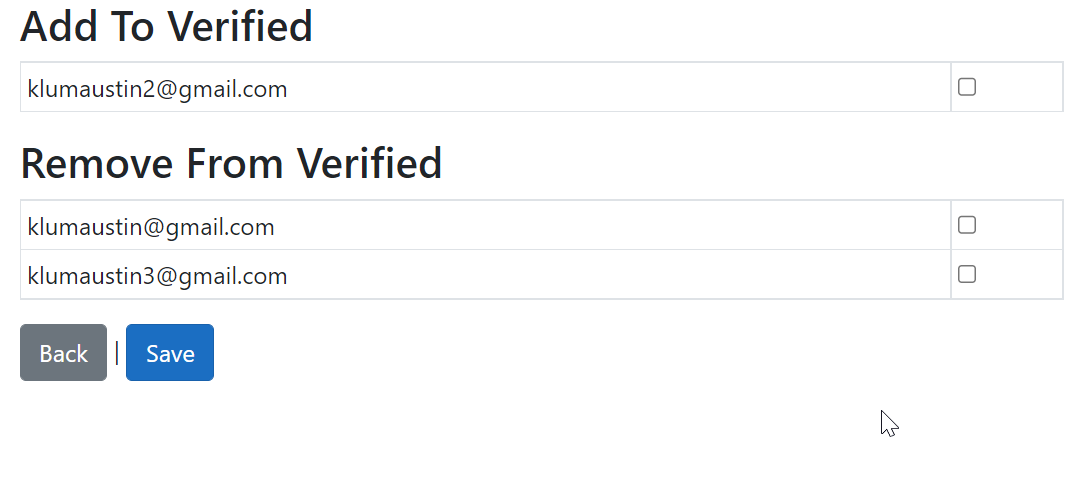
\includegraphics[width=.6\textwidth]{Requirements/assets/cc-add-verified-user.png}
	\caption[Course Creator - Verify Users Page]{\label{CC Verify}Course Creator - Verify Users Page}
\end{figure}
Once a user is verified and completes logging in, they will see a list view of all the created courses. From this page a verified user is able to view, create, update, and delete courses. Figure \ref{CC All Courses} shows the list view of the existing courses. 
 \begin{figure}[htb]
 	\centering
 	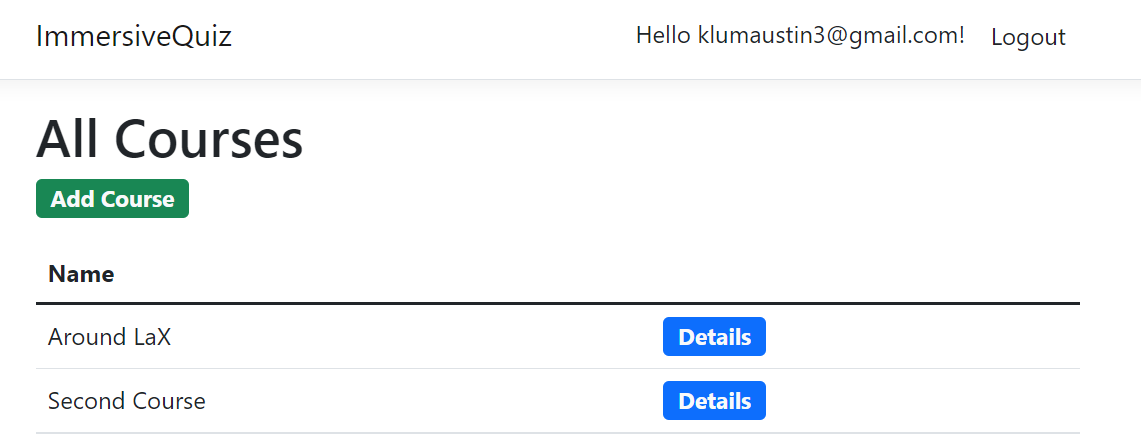
\includegraphics[width=.6\textwidth]{Requirements/assets/cc-all-courses.png}
 	\caption[Course Creator - Veiw All Courses]{\label{CC All Courses}Course Creator - View All Courses}
 \end{figure}
Upon clicking the ``Add Course" button a verified user will be taken to the Course Create screen. A course is simply a named container for all the locations, questions, and answers. While not pictured the create screens for questions and answers are also similar. Figure \ref{CC Create Course} shows the Course Create screen.
\begin{figure}[htb]
	\centering
	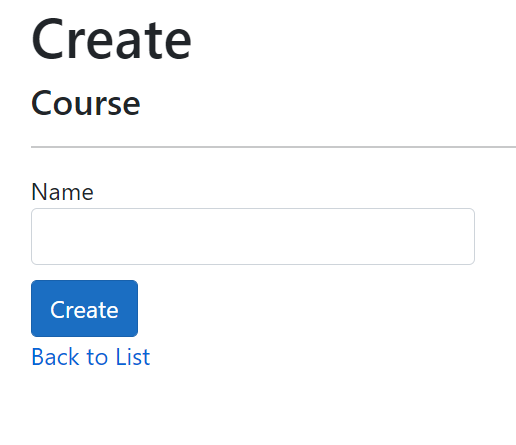
\includegraphics[width=.6\textwidth]{Requirements/assets/cc-create-course.png}
	\caption[Course Creator - Create Course Screen]{\label{CC Create Course}Course Creator - Create Course Screen}
\end{figure}
Once a course is created, a verified user can click the ``Details" button on a course from the list view which loads the Course Details screen. The Course Details shows all of the locations, questions, and answers for a course in expandable dropdowns. The location dropdown also shows a preview of the image and a link to view the full image in a new tab. Figure \ref{CC Course Dashboard} shows the details of the Around LaX course. Figure \ref{CC Expanded} shows the expansion of the questions on a given location. 
\begin{figure}[htb]
	\centering
	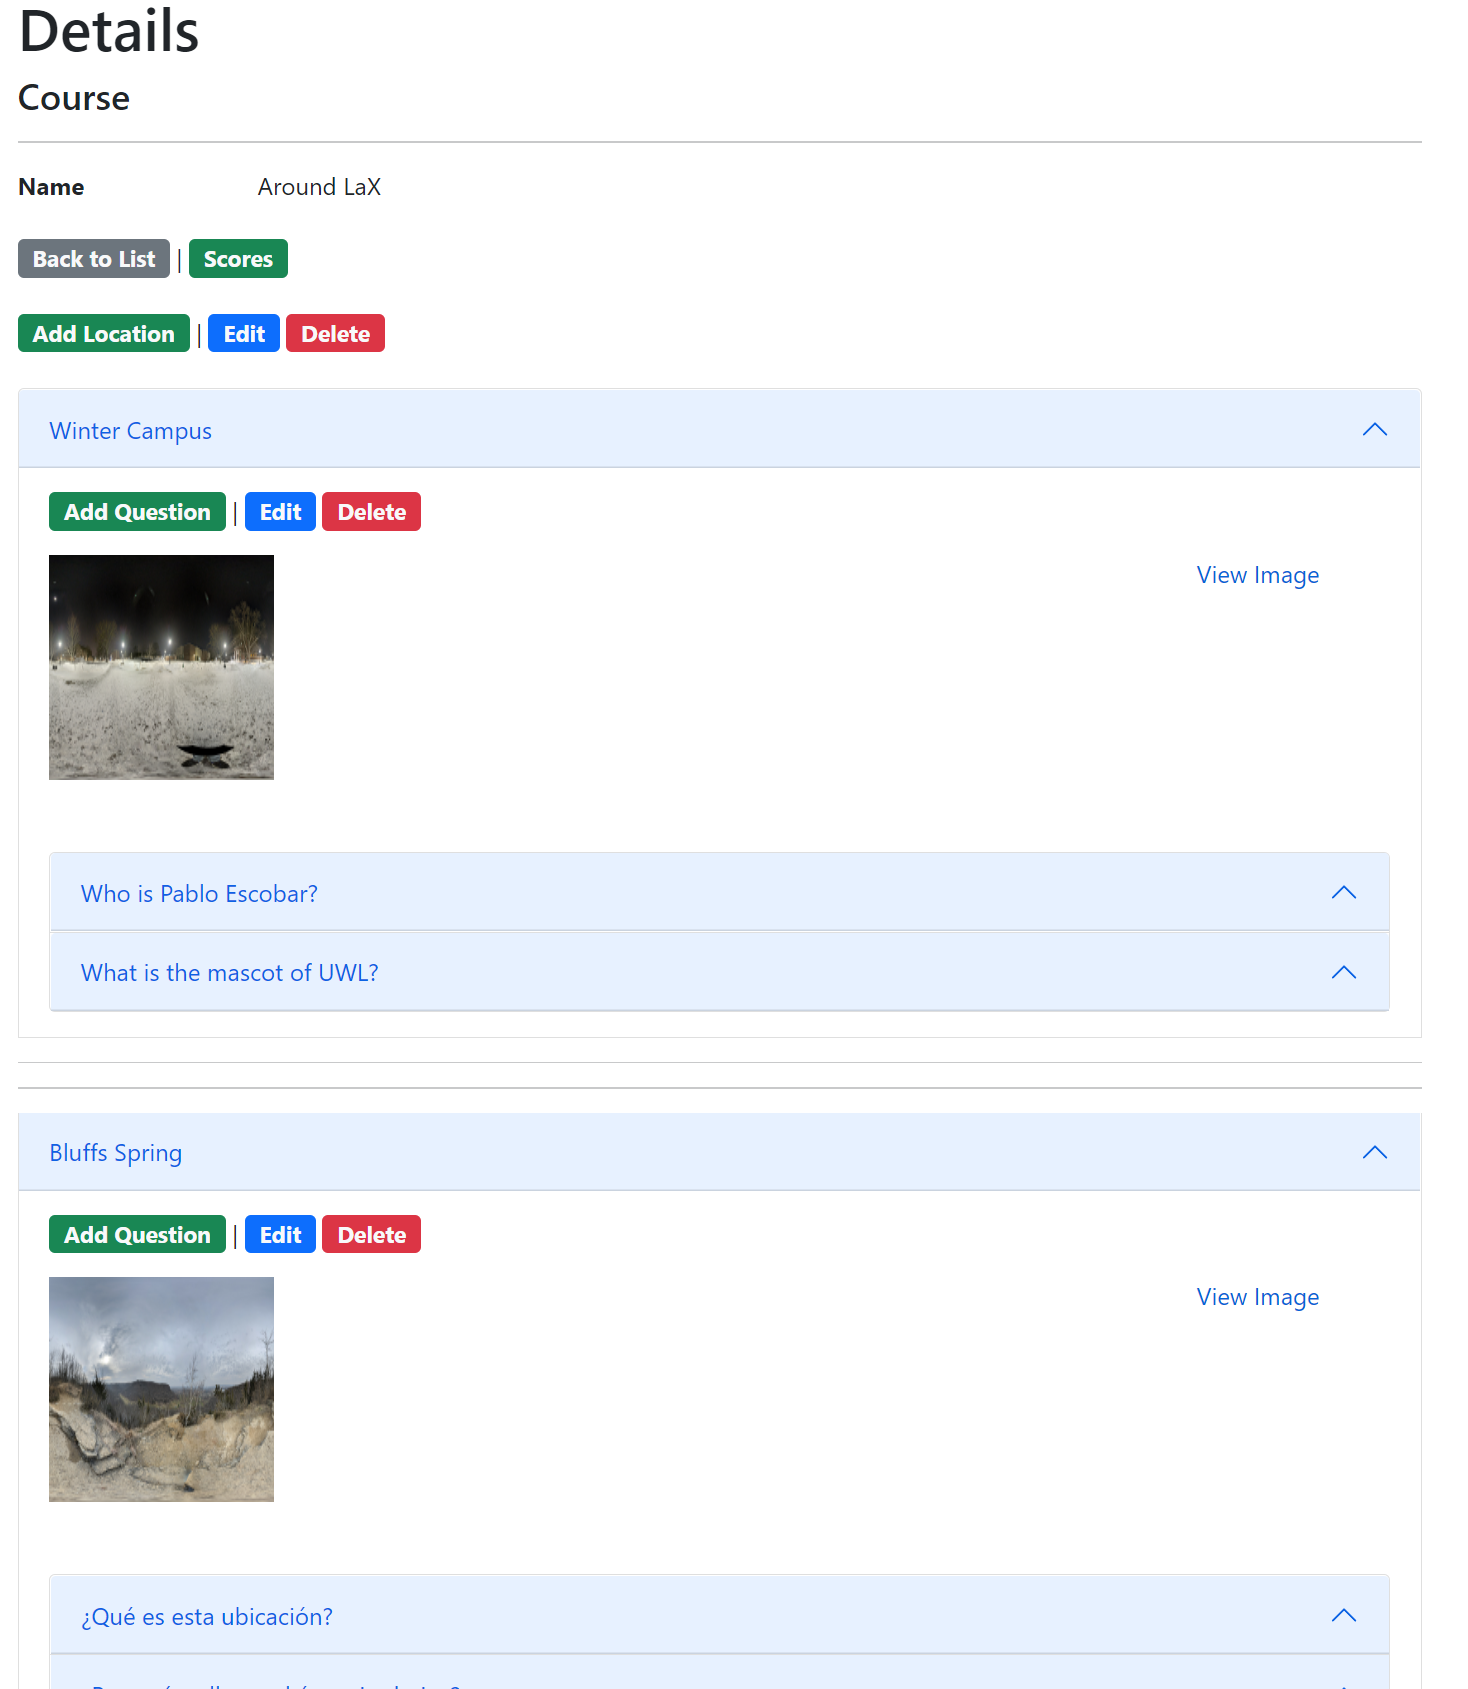
\includegraphics[width=.6\textwidth]{Requirements/assets/cc-course-dashboard.png}
	\caption[Course Creator - Course Details Screen]{\label{CC Course Dashboard}Course Creator - Course Details Screen}
\end{figure}
\begin{figure}[htb]
	\centering
	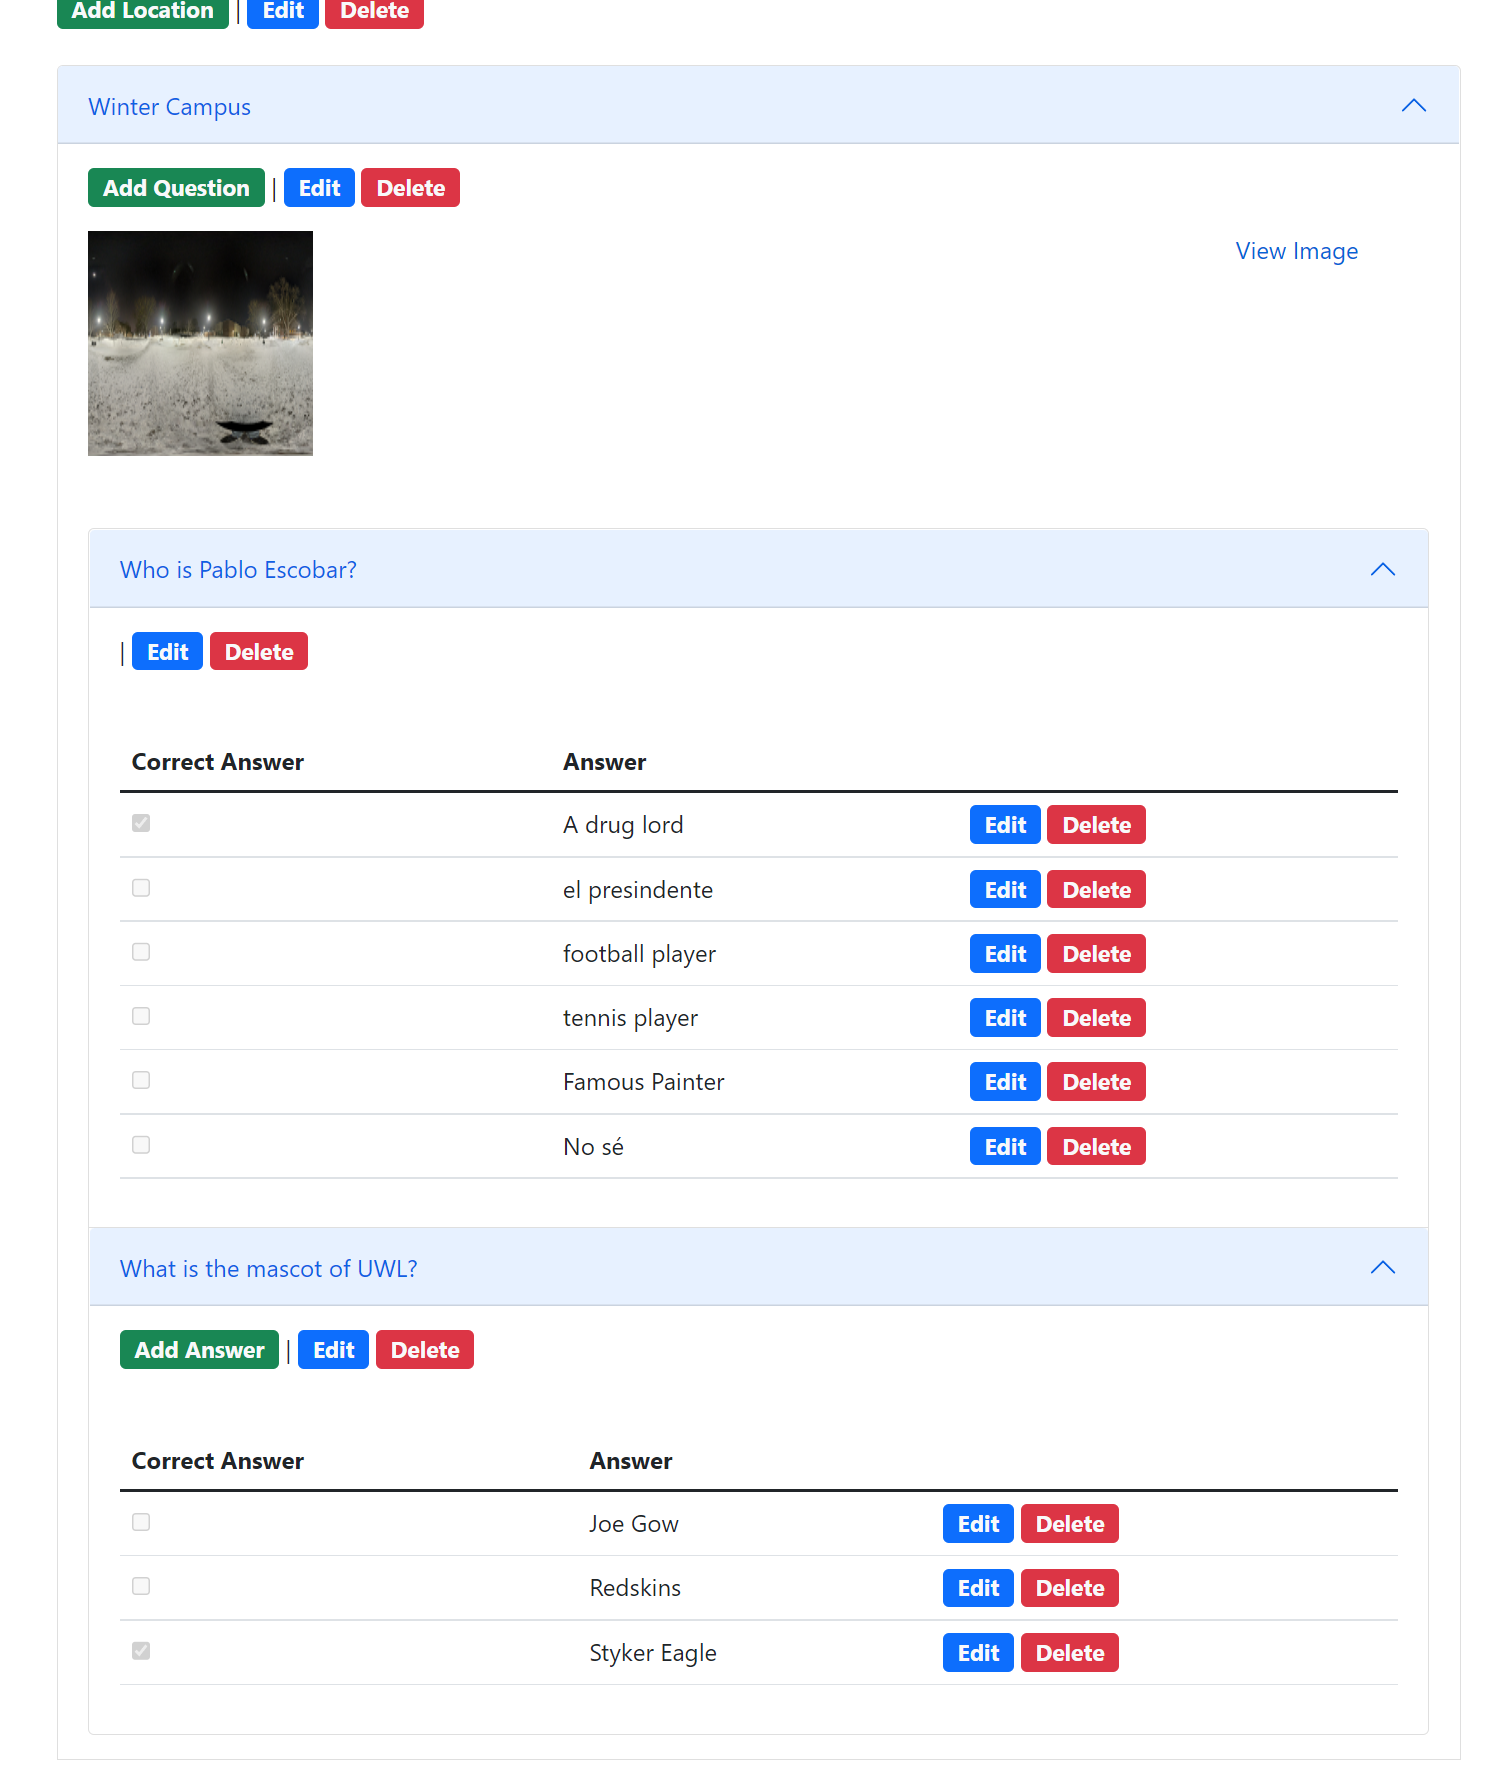
\includegraphics[width=.6\textwidth]{Requirements/assets/cc-questions-expanded.png}
	\caption[Course Creator - Course Details Expanded Questions]{\label{CC Expanded}Course Creator - Course Details Expanded Questions}
\end{figure}
To create a new location, a verified user clicks on the ``Add Location" button which loads the Create Location screen. The Create Location screen contains the location name and a file uploader for the 360 photo of the location. Figure \ref{CC Create Location} shows the Create Location screen.
\begin{figure}[htb]
	\centering
	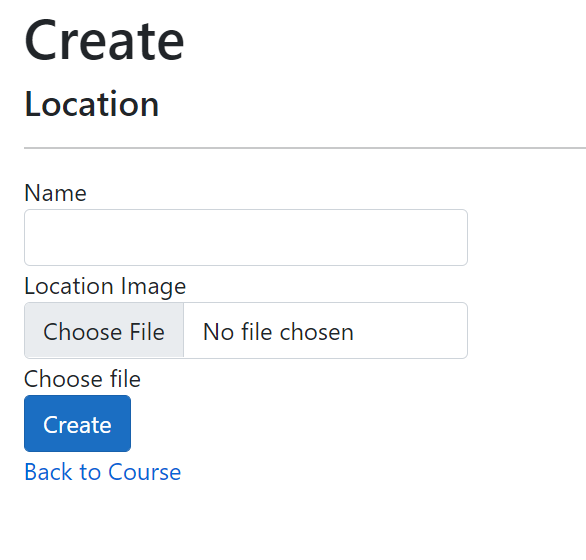
\includegraphics[width=.6\textwidth]{Requirements/assets/cc-create-location.png}
	\caption[Course Creator - Create Location Screen]{\label{CC Create Location}Course Creator - Create Location Screen}
\end{figure}
All of the components of a course are editable. The edit of a course, location, and question are all similar with the current value filled in and the ability to edit the value and save. The edit of an answer is more interesting including the answer content and a checkbox for a ``Is Correct" answer. A verified user can click the ``edit" button on any of these components to bring up the corresponding edit screen. Figure \ref{CC Edit Answer} shows an answer being edited. 
\begin{figure}[htb]
	\centering
	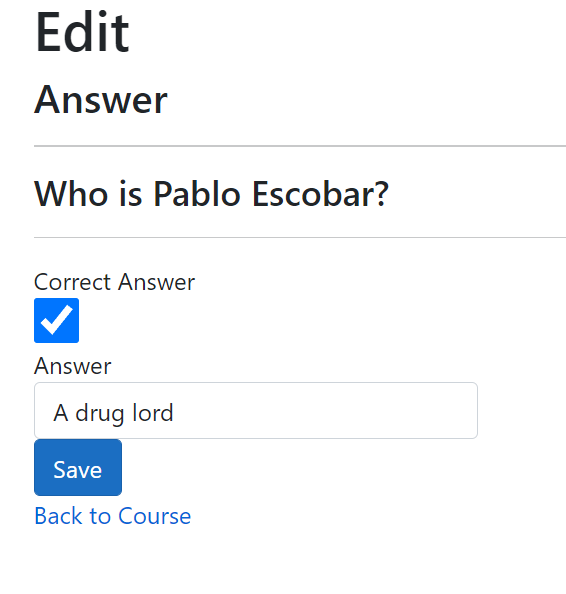
\includegraphics[width=.6\textwidth]{Requirements/assets/cc-edit-answer.png}
	\caption[Course Creator - Edit Answer Screen]{\label{CC Edit Answer}Course Creator - Edit Answer Screen}
\end{figure}
Along with being editable, all components are deletable. The delete of a course, location, question, and answer are all similar. A verified user can click the ``Delete" button to delete a component. A confirmation screen is loaded describing the action the user is about to take. Upon deletion all corresponding subcomponents are also deleted. An example of this would be deleting a course, which would also delete the locations, questions, and answers related to the course. Figure \ref{CC Delete Course} shows the confirmation screen of deleting a course.
\begin{figure}[htb]
	\centering
	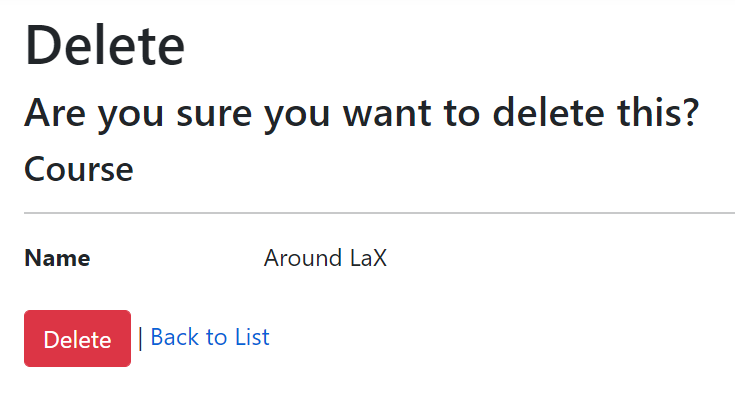
\includegraphics[width=.6\textwidth]{Requirements/assets/cc-delete-course.png}
	\caption[Course Creator - Delete Course Screen]{\label{CC Delete Course}Course Creator - Delete Course Screen}
\end{figure}
Once a course is completed by a student the results are viewable in the Course Score screen. A verified user can click the ``Scores" button to view the related scores for a course. The Scores view lists the results of the students who have taken the course. A verified user is also able to create, edit, and delete scores. Figure \ref{CC Scores} shows the Score screen for the Around LaX course.
\begin{figure}[htb]
	\centering
	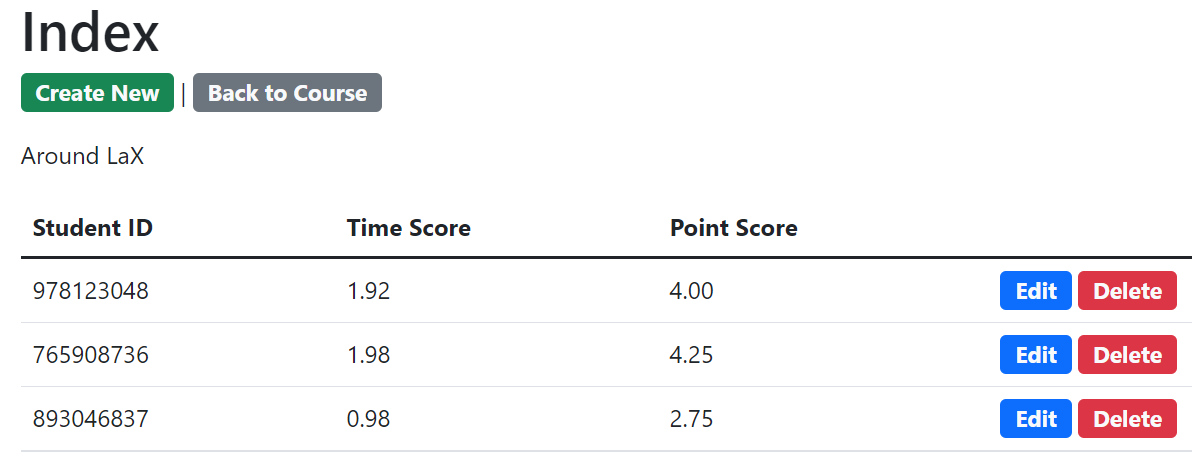
\includegraphics[width=.6\textwidth]{Requirements/assets/cc-score-viewer.png}
	\caption[Course Creator - Course Scores Screen]{\label{CC Scores}Course Creator - Course Scores Screen}
\end{figure} 
Once a user is finished using the Course Creator program, they are able to logout by clicking the ``Logout" button on the top toolbar. This destroys the user's session and will require the user to log back in to use the Course Creator again.
\subsection{Virtual Reality Orienteering}
This tool is used by the students to complete the created orienteering courses that the project sponsor or verified user(s) created. Upon starting the program the user is prompted to enter their student ID using a ``mallet" and tap virtual keyboard. Once the student has entered their student ID, they then select the course via a select list with a point and trigger arrow pointers buttons. After hitting the start button the student begins the course. The first location is loaded up and the student can look around the location. Upon touching the touch pad the first question and corresponding possible answers appears in the world view. As part of the orienteering spirit each question must be answered correctly to continue on to the next question. When a student answers incorrectly the button turns red and is disabled. When answered correctly the button flashes green and the next question and corresponding possible answers load. The student is graded on how quickly they came to the correct answer and, with the orienteering aspect in mind, the time to completely answer all the questions in a location. Each question is worth one point and each location time is worth one point. The score point is awarded divided by the number of attempts. This means that a question with four possible answers the following outcomes are possible: answered correctly has one point awarded, one incorrect attempt has .75 points awarded, two incorrect attempts has .5 points awarded, and three incorrect attempts has .25 points awarded. For the time aspect of the grade, the student has 100 seconds to complete the location, where each second is worth .01 points. This means if the student took 30 seconds to answer the questions and complete the location, they are awarded with .70 points. A time of 45 seconds is awarded .65 points. \\
\\
Upon answering all the questions for a location, the next location is loaded and the timer is reset. Once all locations have been completed a game over screen appears stating the student's point score, time score, total score, and what the maximum points awarded could be. 
\subsubsection{Users}
Figure \ref{Virutal Reality Orienteering Use Case Diagram} shows the use case diagram for the Virtual Reality Orienteering program.

\begin{figure}[h]
	\centering
	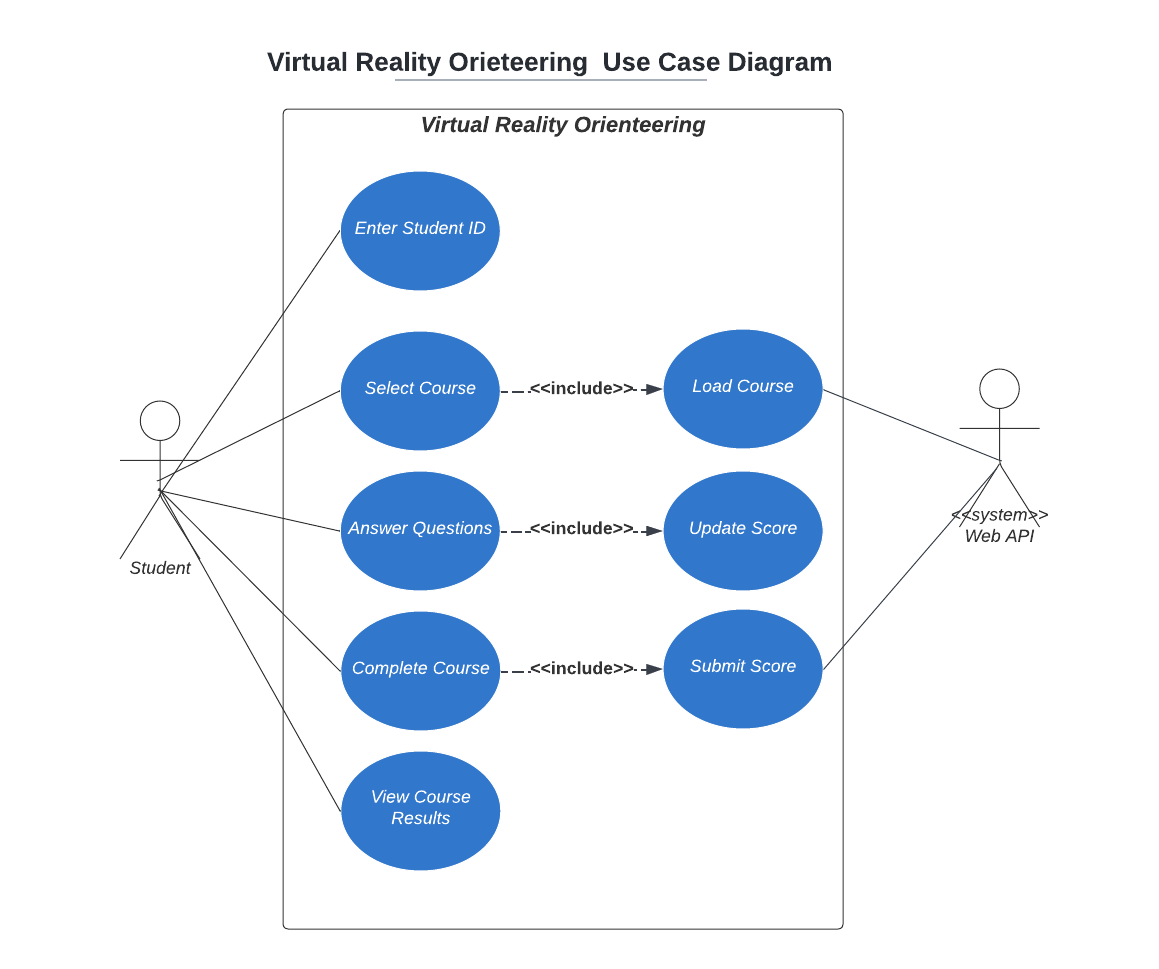
\includegraphics[width=.9\textwidth]{Requirements/assets/vr-use-case-diagram.png}
	\caption[Virutal Reality Orienteering Use Case Diagram]{\label{Virutal Reality Orienteering Use Case Diagram}Virtual Reality Orienteering Use Case Diagram}
\end{figure}

\subsubsection{Virtual Reality Orienteering Flow}
To complete a course a student must start the Virtual Reality Orienteering program and put on a Virtual Reality headset. The student is then prompted to enter in their student ID using a virtual keyboard and a ``Mallet" input system. Figure \ref{VR Keyboard} shows the virtual keyboard and ``Mallet" input system.
\begin{figure}[h]
	\centering
	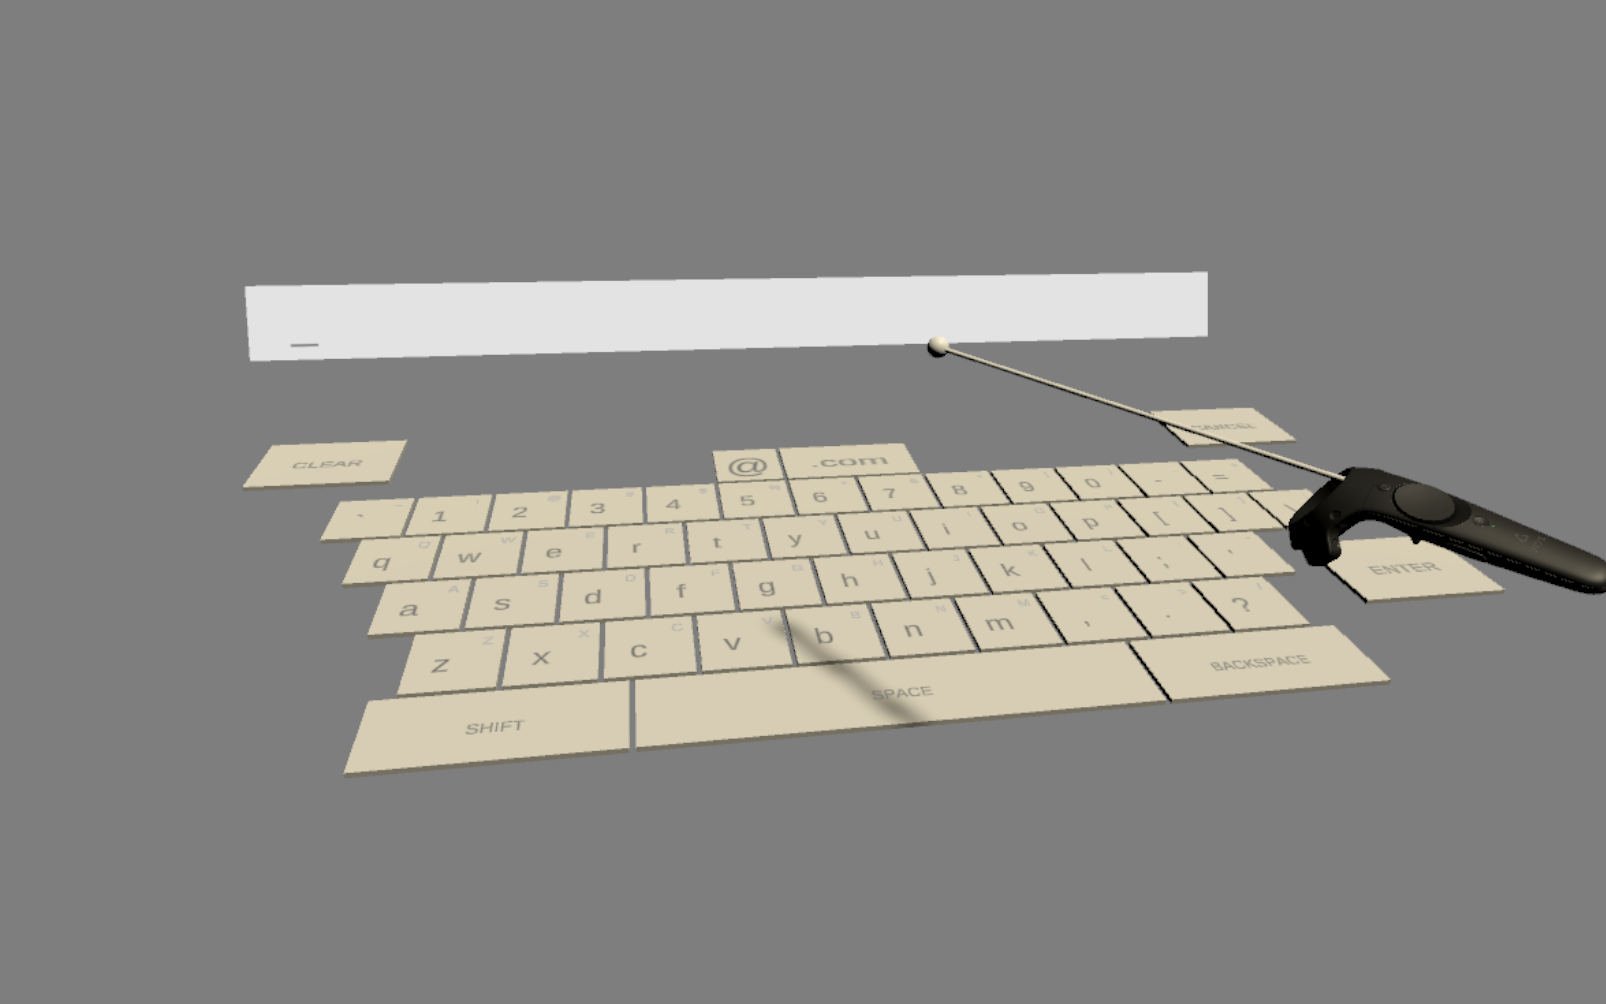
\includegraphics[width=.6\textwidth]{Requirements/assets/vr-keyboard.png}
	\caption[Virtual Reality Orienteering - Student ID Keyboard]{\label{VR Keyboard}Virtual Reality Orienteering - Student ID Keyboard}
\end{figure}
Once a student has entered their student Id, the Course Selector screen appears. The Course Selector screen is a list of all possible courses served up by a call to the Web API. The student is able to use a point and trigger input system to move up or down the list with the corresponding buttons. Once a desired course is picked the student clicks the ``Start" button to begin the course.\\
\\
Upon starting a course the 360 photo of the first location is loaded. The timer for the each location starts upon loading a new location. The student is able to look around the worldspace to promote an immersive experience. Figure \ref{VR Worldspace} shows the student looking around the location in the worldspace. 
\begin{figure}[htb]
	\centering
	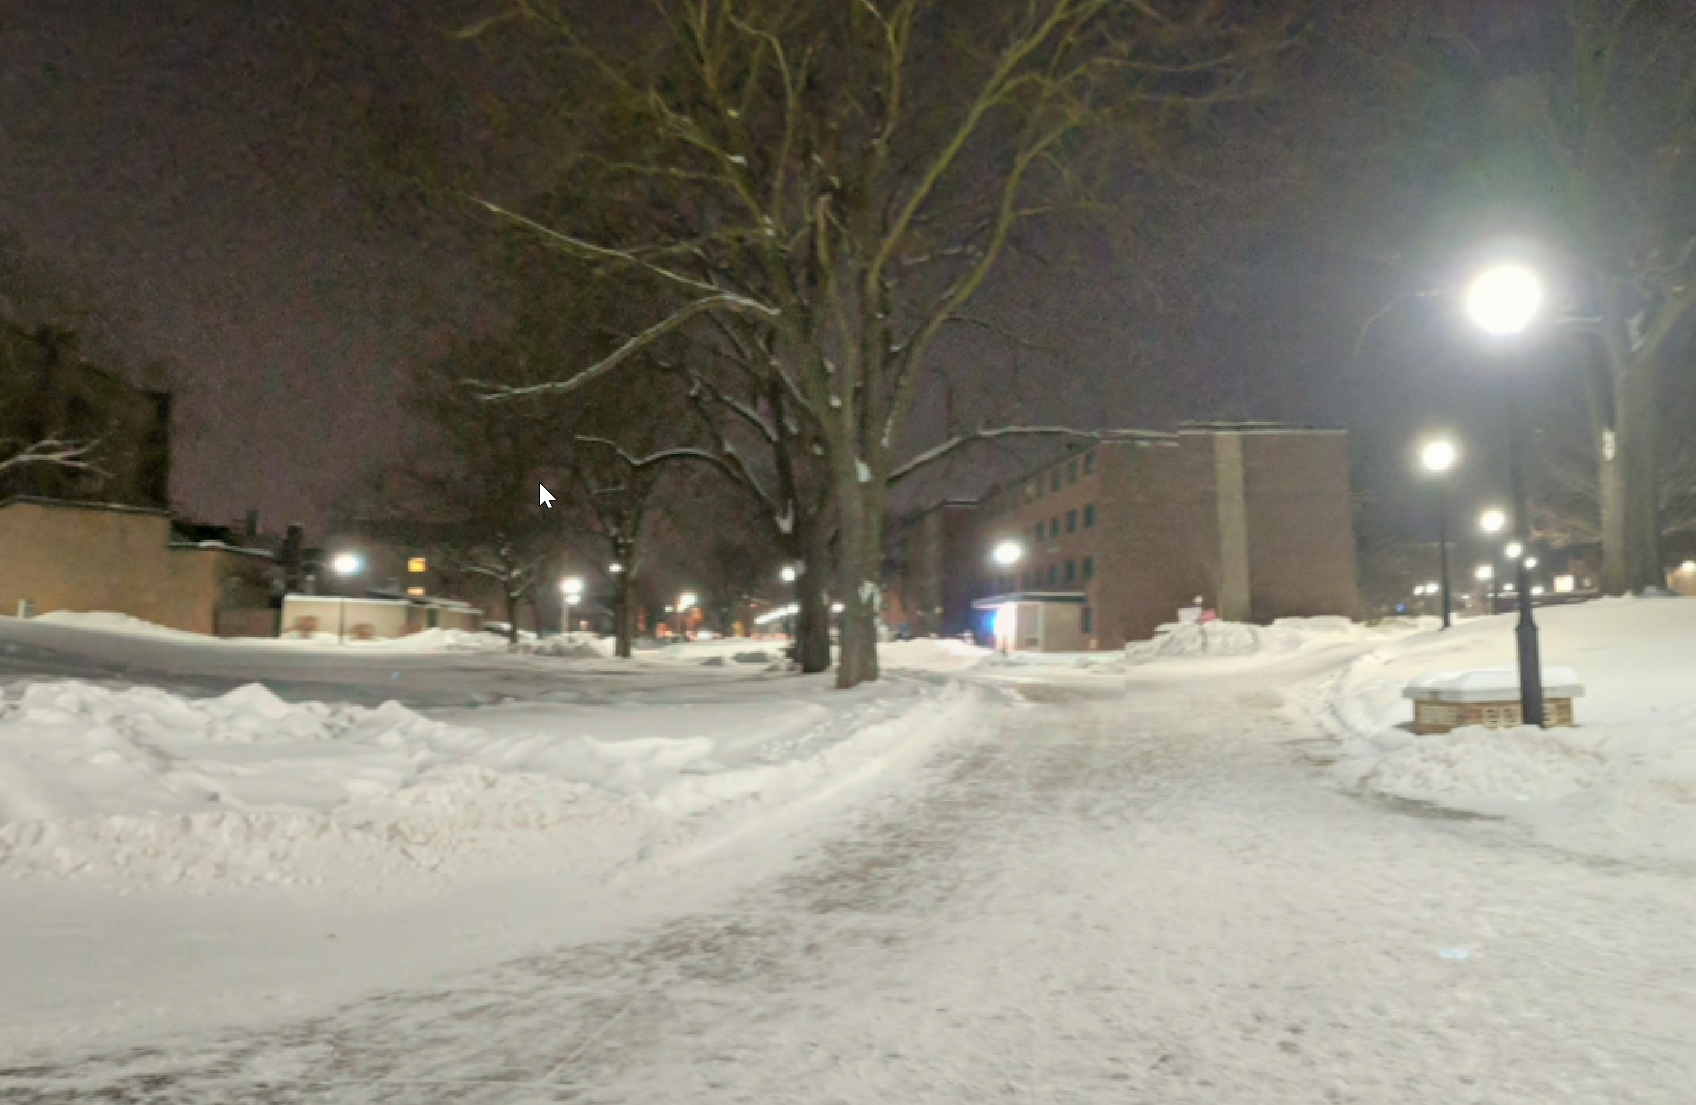
\includegraphics[width=.6\textwidth]{Requirements/assets/vr-worldspace.png}
	\caption[Virtual Reality Orienteering - Veiwing Worldspace]{\label{VR Worldspace}Virtual Reality Orienteering - Viewing Worldspace}
\end{figure}
Once the student has looked around and is satisfied that they know the location, they are able to press the touchpad and load up the questions screen. The question screen is populated by a call to the Web API. A student is able to answer the questions by using the point and trigger input system and the corresponding answer buttons. Figure \ref{VR Question} shows the student looking at the questions screen and hovering over a answer button. 
\begin{figure}[htb]
	\centering
	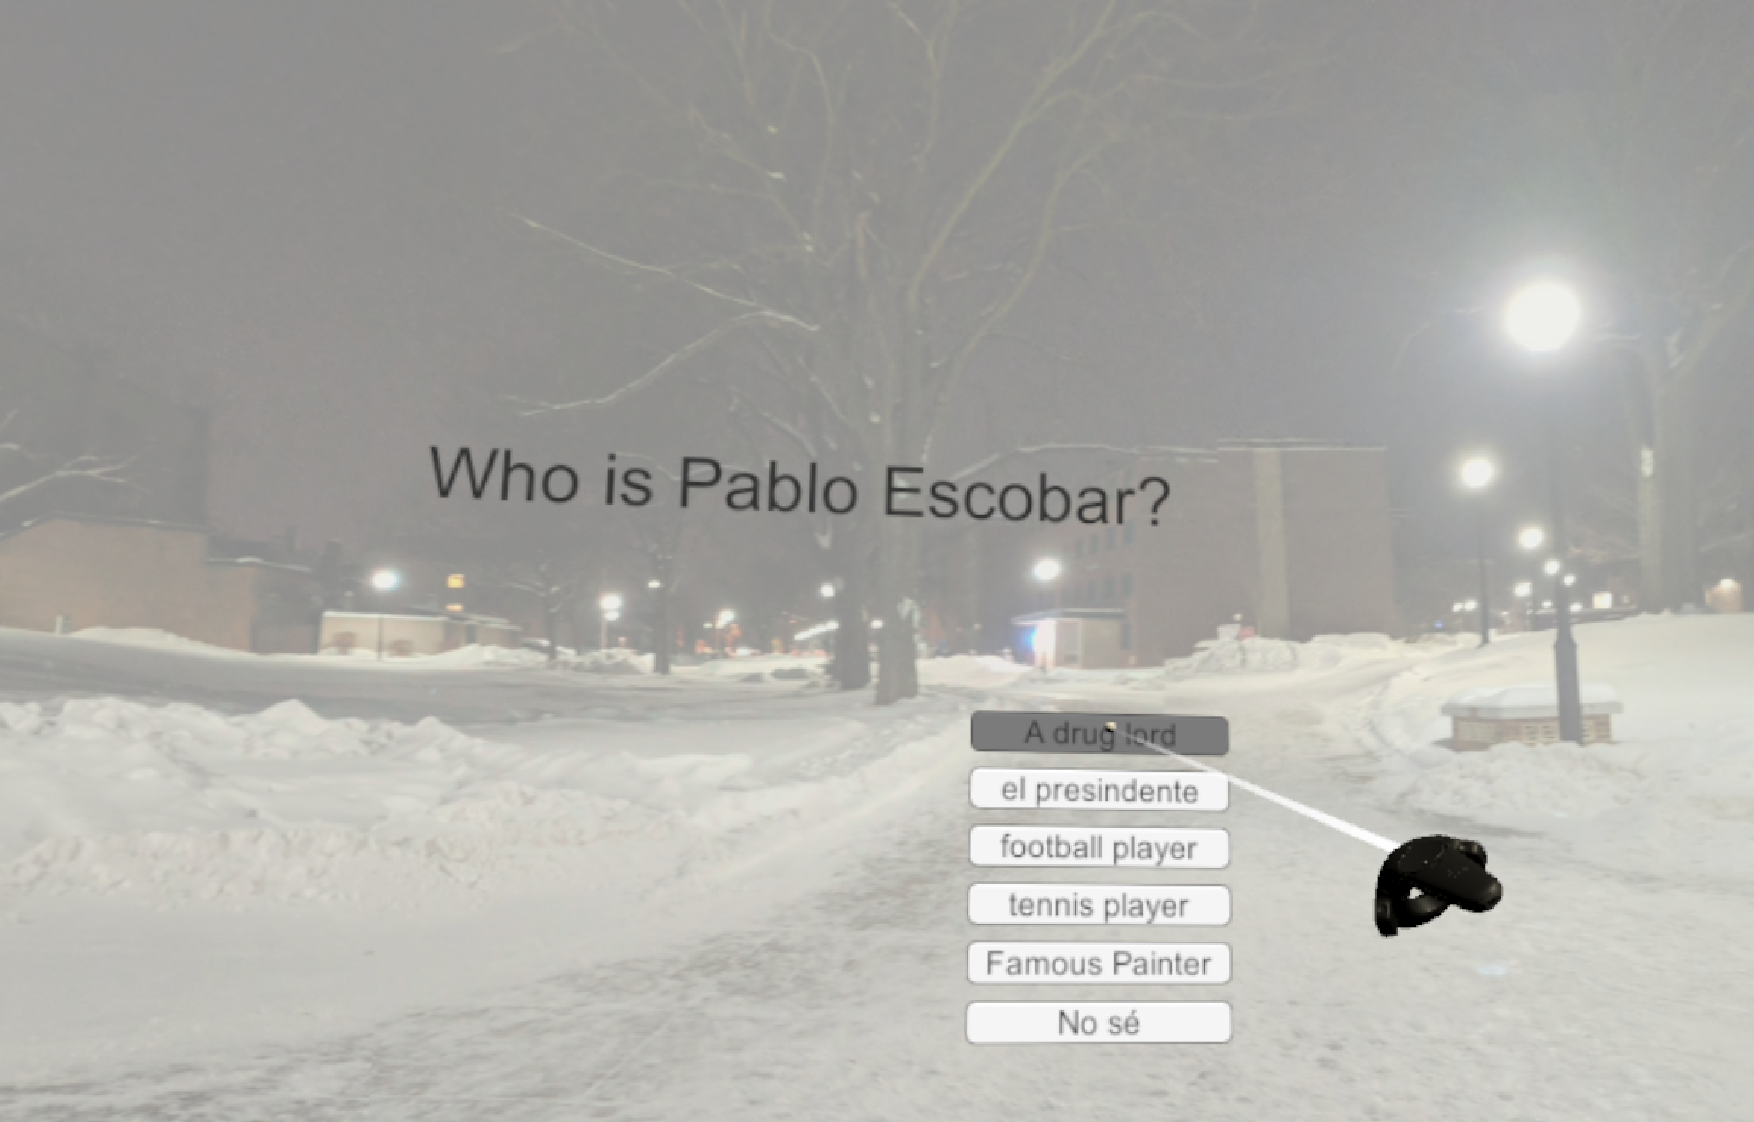
\includegraphics[width=.6\textwidth]{Requirements/assets/vr-view-questions.png}
	\caption[Virtual Reality Orienteering - Questions Screen]{\label{VR Question}Virtual Reality Orienteering - Questions Screen}
\end{figure}
When a student answers incorrectly, their point score is subtracted and the answer button turns red to indicate an incorrect answer. Upon answering correctly the answer button flashes green and the next question is loaded. Figure \ref{VR Incorrect Answer} shows a student who answered a question incorrectly twice with two red answer buttons indicating an incorrect answer.
\begin{figure}[htb]
	\centering
	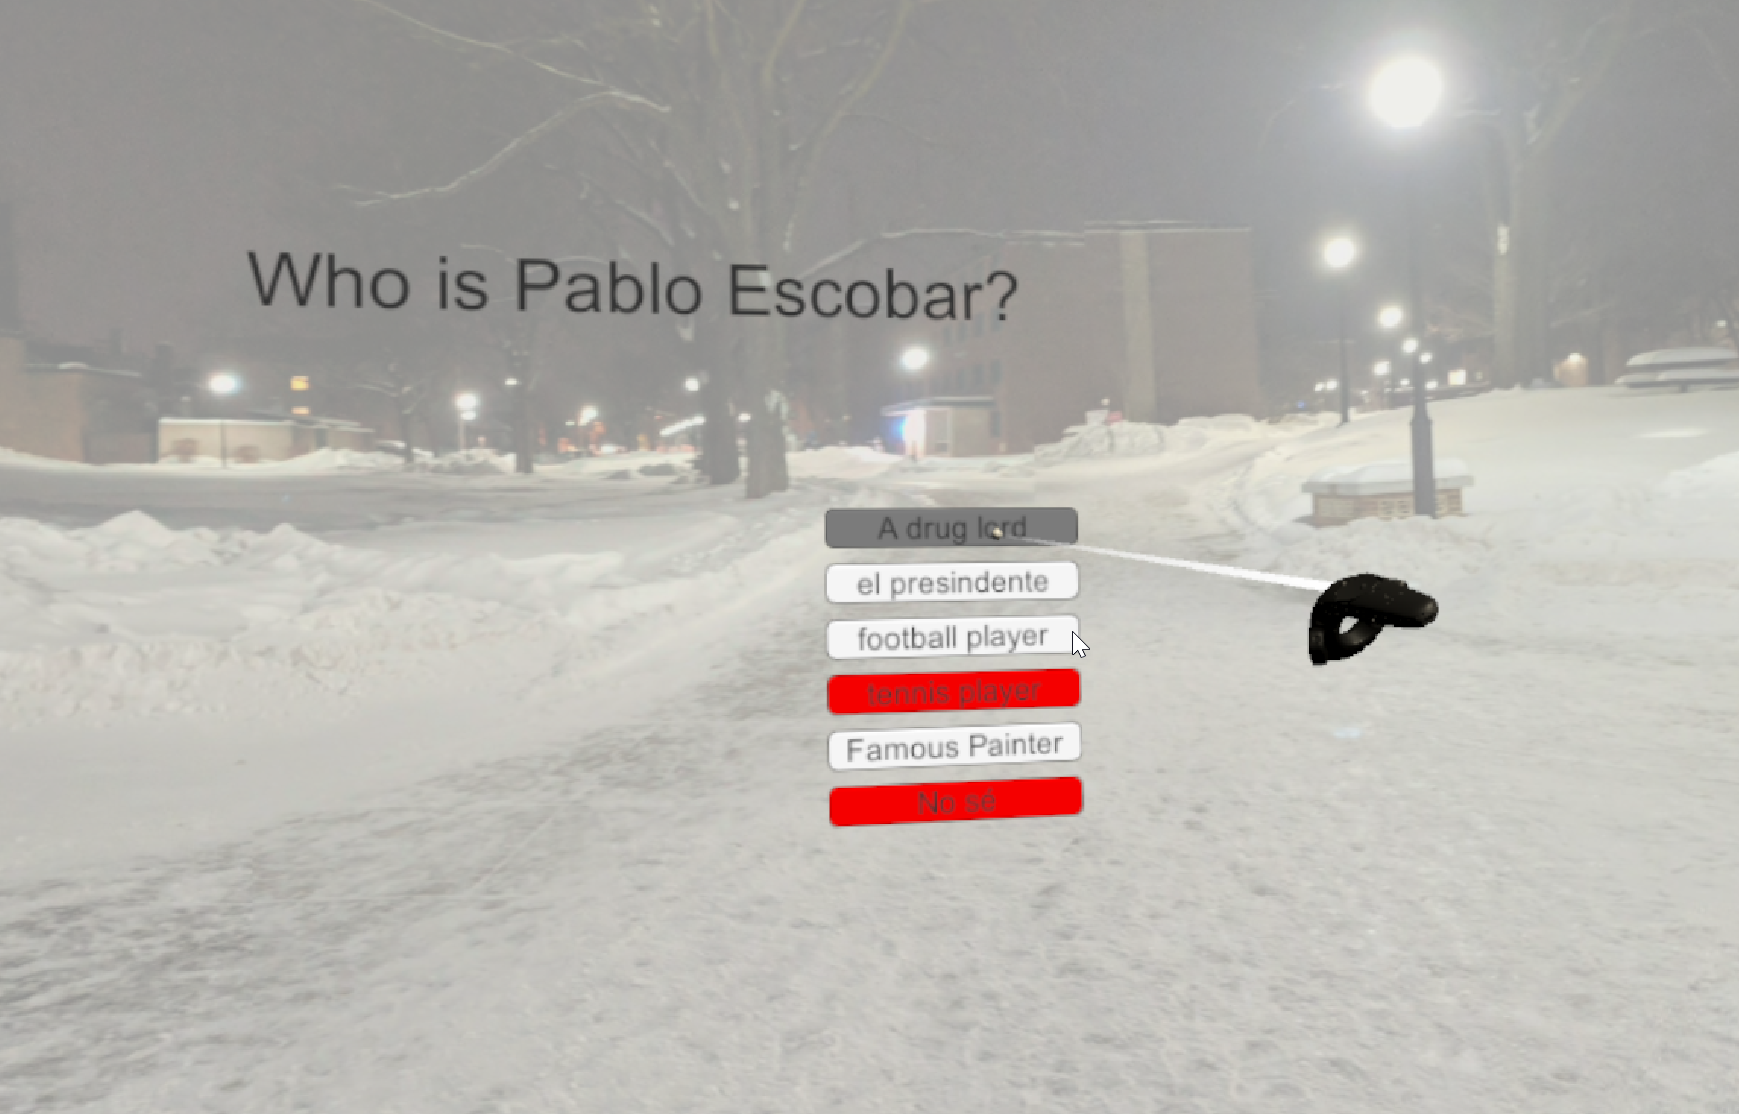
\includegraphics[width=.6\textwidth]{Requirements/assets/vr-answer-incorrectly.png}
	\caption[Virtual Reality Orienteering - Incorrect Answers]{\label{VR Incorrect Answers}Virtual Reality Orienteering - Incorrect Answers}
\end{figure}
The student continues answering the questions until all are answered correctly. Once all questions are answered, the next location is loaded with the new 360 photo loaded into the worldspace. The timer is reset upon loading the new location. Again, once the student is satisfied they know the location they are able to press the touchpad and answer the questions for the corresponding location. This continues on until all locations and corresponding questions are answered. Once all locations are completed a game over screen is displayed presenting the student with their point and time score. The score is submitted to the Course Creator database via another call to the Web API. Figure \ref{VR Game Over} shows an example game over screen with the point and time score presented. 
\begin{figure}[htb]
	\centering
	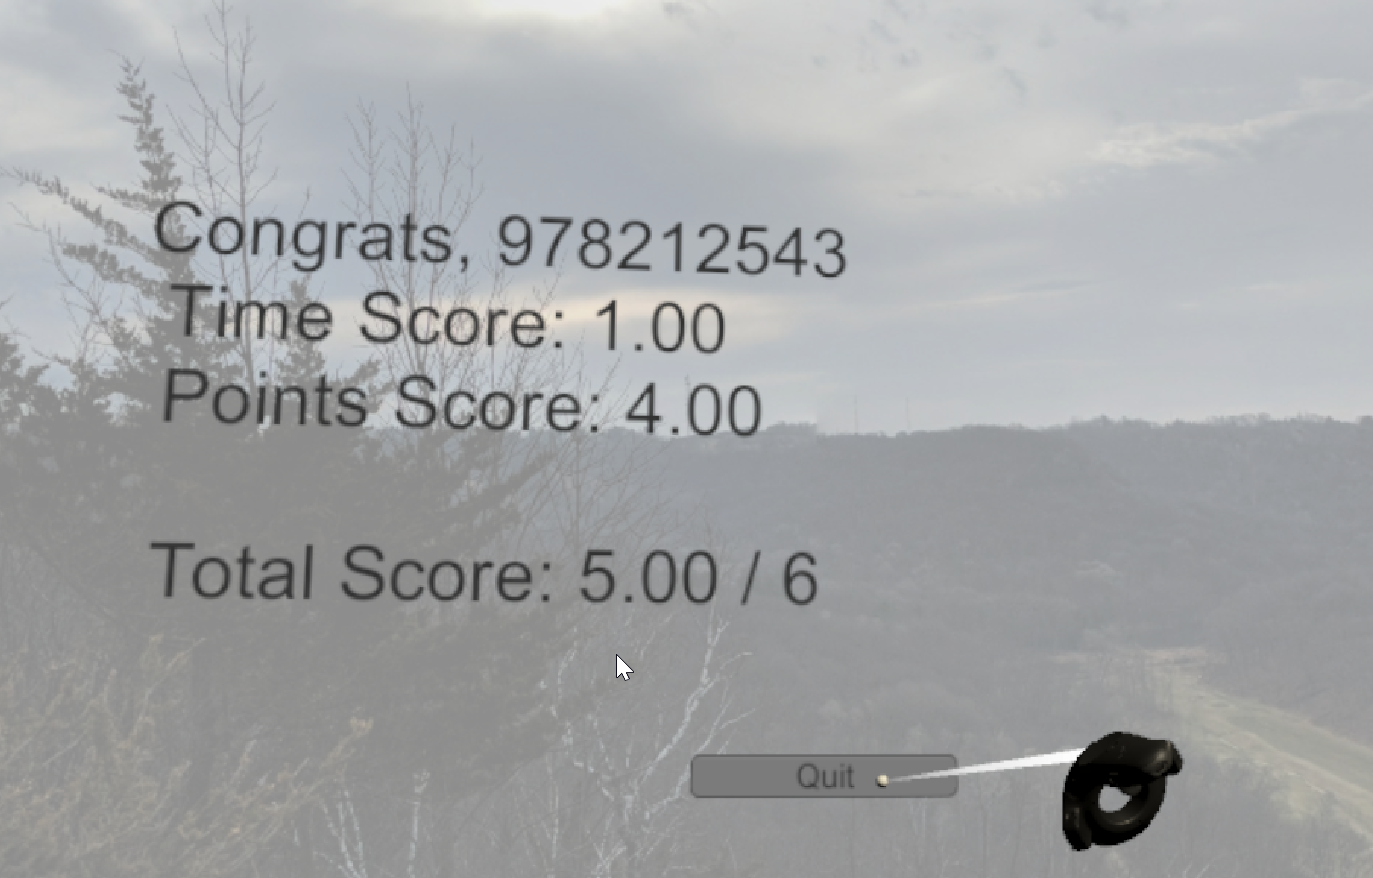
\includegraphics[width=.6\textwidth]{Requirements/assets/vr-game-over.png}
	\caption[Virtual Reality Orienteering - Game Over]{\label{VR Game Over}Virtual Reality Orienteering - Game Over}
\end{figure} 
The student is able to exit the Virtual Reality Orienteering program by using the point and trigger input system to click the ``Quit" button.
\subsection{Functional Requirements}
Functional requirements describe what the system does. These are hard functionalities that the system must provide in order to be considered complete. The following are the high-level functional requirements for this project described from the viewpoint of the users:
\begin{itemize}
	\item As a user, I would like to\ldots
	\begin{itemize}
		\item register an account
		\item login and logout of my account
		\item edit my account information
	\end{itemize}
	\item As a verified user, I would like to\ldots
	\begin{itemize}
		\item view, create, update, and delete courses
		\item view, create, update, and delete locations
		\item view, create, update, and delete questions
		\item view, create, update, and delete answers
		\item view the list of courses
		\item view course results
		\item verify other users
	\end{itemize}
	\item As a student, I would like to\ldots
	\begin{itemize}
		\item enter my student ID  within a VR experience
		\item select a course within a VR experience
		\item complete a orienteering course within a VR experience
	\end{itemize}
\end{itemize}

\subsection{Non-functional Requirements}
Non-functional requirements describe how a system preforms its required functions. These describe the qualities that the system should aim for. The following are the high-level non-functional requirements for this project:
\begin{itemize}
	\item The project should be open-sourced
	\item The project should be cross-platform supported
	\item The project should securely store student result information
	\item The project should securely transmit student results between the two programs
	\item The project should be light-weight and portable
	\item The Virtual Reality Orienteering program should promote immersion and cultural understanding
	\item The Course Creator program should be easy and intuitive to use
	\item The Course Creator should require proper authorization and authentication policies
	\item The Course Creator should validate user input and display the errors in a user friendly message
\end{itemize}